% !TeX spellcheck = en_GB
\documentclass[10pt,letterpaper,oneside]{article}
\usepackage{fontspec}
\usepackage{arev}
\usepackage[utf8]{inputenc}
\usepackage[T1]{fontenc}
\usepackage{amsmath}
\usepackage{amsfonts}
\usepackage{amssymb}
\usepackage{graphicx}
\usepackage{csquotes}
\usepackage{booktabs}
\usepackage{multicol}
\usepackage{enumerate}
\usepackage{microtype}
\usepackage[labelfont=bf,font={small}]{caption}
\usepackage{hyperref}
\usepackage{booktabs}
\usepackage{subcaption}
\usepackage{fancyhdr}
\usepackage[svgnames]{xcolor}
\usepackage{mdframed}
\usepackage{multicol}
\usepackage[para]{footmisc}
\usepackage{siunitx}
\usepackage{cleveref}
\usepackage{listings}
\usepackage{cprotect}


\lstset{ % General setup for the package
	language=Python,
	basicstyle=\small\ttfamily,
	tabsize=4,
	columns=fixed,
	showstringspaces=false,
	showtabs=false,
	keepspaces,
	commentstyle=\color{SeaGreen},
	keywordstyle=\bf\ttfamily\color{DarkBlue}
}

\newfontfamily\symbolfont{Symbola}
\usepackage[left=1in,right=1in,top=1in,bottom=1in,marginparwidth=0.3in]{geometry}

\usepackage[sorting=none]{biblatex}
\addbibresource{../bibliography.bib}

\author{Andreas Stöckel\\[0.5cm]Based on lecture notes by\\Chris Eliasmith and Terrence~C.~Stewart}
\newcommand{\baseCodeURL}{https://github.com/astoeckel/syde556-w20/blob/master/lectures}

\fancyhf{}
\fancyhead[L]{SYDE 556/750 Lecture Notes}
\fancyhead[R]{Andreas Stöckel}
\fancyfoot[C]{\thepage}
\pagestyle{fancy}

\setlength{\parindent}{0em}
\setlength{\parskip}{0.5em}
\renewcommand{\baselinestretch}{1.25}
\renewcommand{\vec}[1]{{\mathbf{#1}}}
\newcommand{\mat}[1]{{\mathbf{#1}}}
\newcommand{\T}{\ensuremath{\mathrm{T}}}
\renewcommand{\epsilon}{\varepsilon}
\renewcommand{\phi}{\varphi}

\makeatletter
\newcommand{\superimpose}[2]{%
	{\ooalign{{#1}\hidewidth\cr{#2}\hidewidth\cr}}}
\makeatother
\newcommand{\SolidCircle}[2]{\superimpose{\color{#1}\symbolfont ⬤}{\textbf{\color{white}#2}}\hspace{1em}}
\newcommand{\OPlus}{\SolidCircle{DarkGreen}{\kern0.75pt+}}
\newcommand{\OMeh}{\SolidCircle{DarkOrange}{~}}
\newcommand{\OMinus}{\SolidCircle{DarkRed}{\kern2.25pt--}}

\newcommand{\YouTube}[2][Video]{\href{https://youtu.be/#2}{{\symbolfont 📺}~{#1}}%
%\footnote{\url{https://youtu.be/#2}}%
}

\newcommand{\CodeLink}[2][Code]{\href{\baseCodeURL/#2}{{\symbolfont ⌨}~\emph{#1}}}

\newcommand{\MakeTitle}[1]{
\maketitle
\begin{center}
	
\includegraphics[width=0.5\textwidth]{../assets/uwlogo.pdf}\\[1cm]
	{#1}\
\end{center}

\vfill

\thispagestyle{empty}
\setcounter{page}{0}
\newpage

\pagenumbering{roman}
\setcounter{tocdepth}{2}
\tableofcontents
\newpage

\setcounter{page}{0}
\pagenumbering{arabic}}

\reversemarginpar


\newcommand{\ColorBox}[3]{%
	\marginpar{%
		\huge\raisebox{-3ex}{\symbolfont{#1}}%
	}%
	\begin{mdframed}[hidealllines=true,backgroundcolor=#2,innertopmargin=0.25cm,innerbottommargin=0.25cm]%
		{#3}
	\end{mdframed}}

\newcommand{\Note}[1]{\ColorBox{📌}{WhiteSmoke}{\textbf{Note:} #1}}
\newcommand{\Example}[1]{\ColorBox{💡}{WhiteSmoke}{\textbf{Example:} #1}}
\newcommand{\Aside}[1]{\ColorBox{🌟}{WhiteSmoke}{\emph{Aside:} #1}}
\newcommand{\Python}[1]{\ColorBox{🐍}{WhiteSmoke}{#1}}
\newcommand{\Notation}[1]{\ColorBox{\huge$\Sigma$}{WhiteSmoke}{\textbf{Notaton:} #1}}

\newcommand{\ConstructionSite}{\hrulefill {\symbolfont 🚧} UNDER CONSTRUCTION {\symbolfont 🚧} \hrulefill}

\newenvironment{ImportantEqn}[1]{\mdframed\raggedleft\emph{({#1})}\align}{\endalign\endmdframed}

\date{January 14 \& 16, 2020}
\title{SYDE 556/750 \\ Simulating Neurobiological Systems \\ Lecture 3: Representation}


\begin{document}

\MakeTitle{\textbf{Accompanying Readings: Chapter 2 of Neural Engineering}}

\section{Introduction}

\Note{In the last lecture, we had a look at a the Leaky Integrate-and-Fire neuron model as an approximation of the behaviour of biological neurons. In this lecture, we discuss a theory of neural representation. Together with our knowledge about neural responses this forms a theory of what \enquote{the neural code} may be.}

In order to survive in natural environments, animals must build representations of their environment. This includes physical properties, such as the \emph{velocity} and \emph{location} of objects in the vicinity of the animal, what the \emph{colour} of an object is, but also non-physical properties such as whether an object is, \emph{edible}, \emph{alive}, or \emph{dangerous}. Of course such representations are not only limited to objects, but also carry information about the own body (e.g., \enquote{proprioception}, configuration of limbs; location in space), up to abstract thought and emotions.

\begin{mdframed}
\textbf{NEF Principle 1 -- Representation}\\
The claim of the Neural Engineering Framework (NEF) is that the activity of groups (interchangeably \enquote{populations}, or \enquote{ensembles}) of neurons \emph{represents} values via nonlinear encoding and linear decoding.
\end{mdframed}

For now, mostly because it is the easiest to reason about, we shall restrict ourselves to low-level representations of sensory information. In this case, representation is directly evident from the correlation between some external quantity and neural activity.  We already saw some examples of such representations in the first lecture. For example, in the classical Hubel and Wiesel experiment (\YouTube{KE952yueVLA}, \cite{hubel1959receptive}), individual neural activity is correlated with the location and orientation of a bar of light within the visual field. Similarly, in the case of place cells (\YouTube{lfNVv0A8QvI}), neural activity is correlated with the location of the animal in space.

We will first discuss the encoding and decoding of values in a more abstract sense, and then propose a particular mechanism by which values are encoded within neurons in the Neural Engineering Framework. Since \emph{encoding} only takes us half of the way, we also have to discuss \emph{decoding}, i.e.~how we can estimate the original 

\Notation{Scalars, functions are italic letters ($d$, $n$, $N$, $f$,\textellipsis), vectors are bold lowercase letters ($\vec a, \vec e$), matrices are bold uppercase letters ($\mat A$), sets are double-struck uppercase letters ($\mathbb{R}$, $\mathbb{N}$). $\mathbb{A} \rightarrow \mathbb{B}$ denotes a function mapping from the domain $\mathbb{A}$ onto a codomain $\mathbb{B}$.
\allowdisplaybreaks
\begin{align*}
	d &\in \mathbb{N} &&~ \text{Dimensionality of the value represented by a neuron population} \\
	n &\in \mathbb{N} &&~ \text{Number of neurons in a neuron population} \\
	N &\in \mathbb{N} &&~ \text{Number of samples}\\
	\langle \vec x, \vec y \rangle &: \mathbb{R}^k \times \mathbb{R}^k \rightarrow \mathbb{R} &&~ \text{Dot product between two $k$-dimensional vectors $\vec x$ and $\vec y$} \\¸
	G[J]  &: \mathbb{R} \rightarrow \mathbb{R}^+  &&~ \text{Neural response for an input current $J$ (\emph{response curve})} \\
	a_i (\vec x) &: \mathbb{R}^d \rightarrow \mathbb{R}^+ &&~ \text{Neural response of neuron $i$ in a neural population (\emph{tuning curve})}\\
	\vec a(\vec x) &: \mathbb{R}^d \rightarrow (\mathbb{R}^+)^n &&~ \text{Neural response of all neurons in a neural population}\\
	{\vec e}_i &\in \mathbb{R}^d &&~ \text{Encoding vector, or \enquote{preferred direction}, of neuron $i$ in a population}\\
	\alpha_i &\in \mathbb{R} &&~ \text{The $i$-th neuron's gain factor}\\
	J^\mathrm{bias}_i &\in \mathbb{R} &&~ \text{The $i$-th neuron's bias current}\\
	\vec x_j &\in \mathbb{R}^d &&~ \text{$j$-th (out of $N$) input sample} \\
	{\hat{\vec x}}_j &\in \mathbb{R}^{d} &&~ \text{Decoded $j$-th input sample} \\
	\mat X &\in \mathbb{R}^{d \times N} &&~ \text{Matrix of input samples}\\
	\mat A &\in \mathbb{R}^{n \times N} &&~ \text{Matrix of sampled population activities}\\
	\vec d_i &\in \mathbb{R}^{n} &&~ \text{Decoding vector for the $i$-th neuron in the population} \hspace{0.25cm}\\
	\mat D &\in \mathbb{R}^{d \times n} &&~ \text{Decoding matrix}
\end{align*}\vspace{-0.75cm}}

\section{Abstract Representation}

\section{Neural Representation}

\subsection{Neural Tuning Curves}

\subsection{The Encoding Equation}

We can generate tuning curves that qualitatively match both types of tuning curves we have seen above. To this end, we let our value $\vec x$ be a $d$-dimensional vector (where the dimensionality of the represented value $d$ is specific to each neuron population). We can then choose the dot product as a measure of similarity (see note below):
\begin{align*}
	J_i(\vec x) &= \alpha_i \langle \vec x, \vec e_i \rangle + J^\mathrm{bias}_i \,,
\end{align*}
where $\alpha_i$, $J^\mathrm{bias}_i$ are the gain and bias terms for the $i$-th neuron in the population, $\vec e_i \in \mathbb{R}^d$ is the neuron's encoding -- or \enquote{preferred direction vector}, and $\langle \cdot, \cdot \rangle$ denotes the dot product between two vectors. Note that $\vec e_i$ is always normalised to unit length, that is $\|\vec e_i\| = 1$.

\Note{The \emph{dot product} (also: inner product, scalar product) $\langle \vec x, \vec y \rangle$ of two vectors $\vec x, \vec y \in \mathbb{R}^d$ is defined as
	\begin{align*}
	\langle \vec x, \vec y \rangle &= \sum_{i = 0}^d x_i y_i \,.
	\end{align*}
	We implicitly treat all vectors as column vectors; a vector $\vec x \in \mathbb{R}^d$ is implicitly a $d \times 1$ matrix (i.e., a matrix of $d$ rows and a single column). Hence, by the definition of matrix multiplication, the dot product is also given as
	\begin{align*}
	\langle \vec x, \vec y \rangle &= \vec x^\T \vec y  \quad \text{(matrix dimensions: $(1 \times d) \times (d \times 1) \rightarrow 1 \times 1$)}\,.
	\end{align*}
	In particular, note that the dot product can be interpreted as a vector similarity measure. Namely, according to the Euclidean dot product formula
	\begin{align*}
	\langle \vec x, \vec y \rangle &= \cos(\angle(\vec x, \vec y)) \| \vec x\| \| \vec y\| \,,
	\end{align*}
	where $\| \cdot \|$ denotes the standard $L_2$-norm, and $\angle(\cdot, \cdot)$ is the angle inscribed between two vectors. Hence, the dot product is maximal if the angle between the two vectors is zero (they are pointing in the same direction, the cosine is $+1$) and zero if the two vectors are orthogonal. It is minimal (the cosine is $-1$) if the two vectors are pointing in exactly opposite directions.}

Combining the current $J_i(\vec x)$ with the neuron response curve $G[J]$ (where, again, $G$ is specific to each neuron population) yields the encoding equation:
\begin{ImportantEqn}{Encoding Equation}
	a_i(\vec x) &= G\big[J_i(\vec x)\big] = G\big[\alpha_i \langle \vec x, \vec e_i \rangle + J^\mathrm{bias}_i\big] \,.
\end{ImportantEqn}

\subsection{Encoding Equation Examples}

\paragraph{1D Encoder}
In the case of a one-dimensional encoder, the encoding \enquote{vector} can either be $+1$ or $-1$. This corresponds to o neurons that are either more active in the presence of a stimulus (positive encoder), or neurons that are more active in the absence of a stimulus (negative encoder).

\paragraph{2D Encoder}

\begin{figure}
	\begin{subfigure}{0.5\textwidth}
		\centering
		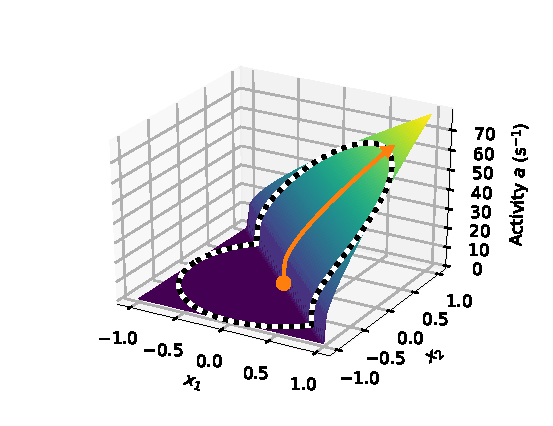
\includegraphics[trim=1cm 0 0 1cm,clip]{media/2d_encoder_tuning_curve.pdf}
		\caption{2D neuron tuning curve}
	\end{subfigure}
	\begin{subfigure}{0.5\textwidth}
		\centering
		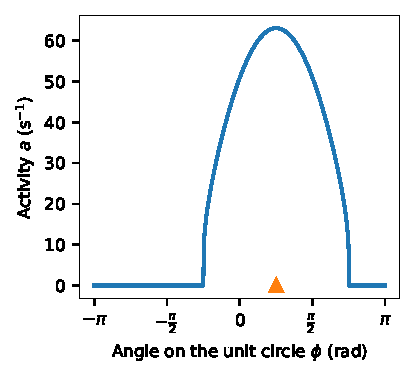
\includegraphics{media/2d_encoder_tuning_curve_unit.pdf}
		\caption{1D projection along the unit circle}
	\end{subfigure}
	\caption{2D neuron tuning curve for the encoding vector $\vec e = (1/\sqrt{2}, 1/\sqrt{2})$. \textbf{(a)} 3D surface plot of the 2D neuron tuning curve. Axes correspond to the magnitude of the first two components of the represented value $\vec x = (x_1, x_2)$. Orange arrow corresponds to the encoding vector. Dotted line corresponds to the unit circle. \textbf{(b)} Neural activity along the unit circle is qualitatively similar to the bell-shaped tuning curves observed in biology. \CodeLink{lecture_03/media/code/2d_encoder.ipynb}}
\end{figure}



\section{Decoding Represented values}

\subsection{Computing Identity Decoders}

\subsection{Decoding Under Noise}

\section{Examples}

\subsection{Horizontal Eye Control (1D)}

\subsection{Arm Movements (2D)}

\subsection{Higher-dimensional Tuning}

\printbibliography

\end{document}
